\subsection{Закон Джоуля-Ленца в интегральной и дифференциальной формах}

\begin{definition}
    Закон Джоуля-Ленца.

    При прохождении по проводнику тока проводник нагревается. Количество тепла, выделяющегося в проводнике пропорционально его сопротивлению, квадрату силы тока и времени прохождения тока.

    $$
    Q=RI^2t
    $$
\end{definition}

\begin{definition}
    Интегральная форма:

    Если сила тока изменяется со временем:

    $$
    Q=\int_0^tRI^2dt
    $$
\end{definition}

При этом силы поля совершают работу:
$\displaystyle dA=Udq=U_idt=RI^2dt$

таким образом, нагревание проводника происходит за счёт работы, совершаемой силами поля над носителями заряда.

\begin{definition}
    Дифференциальная форма:

    $$
    w=\rho j^2=\lambda E^2
    $$
\end{definition}

\begin{figure}[h]
    \centering
    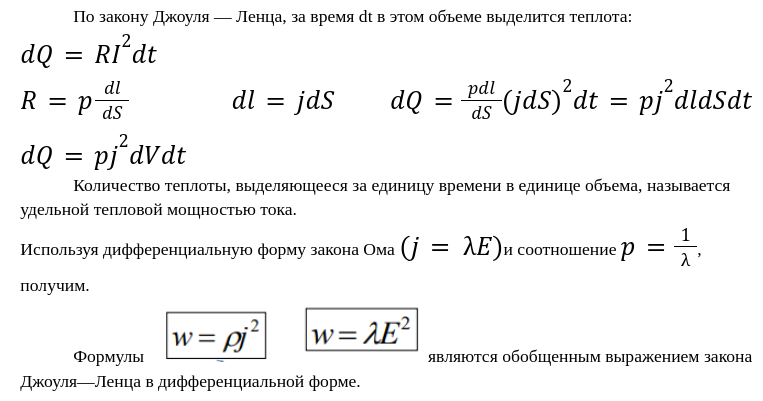
\includegraphics[width=0.7\linewidth]{imgs/q31i1.png}
\end{figure}

\begin{figure}[h]
    \centering
    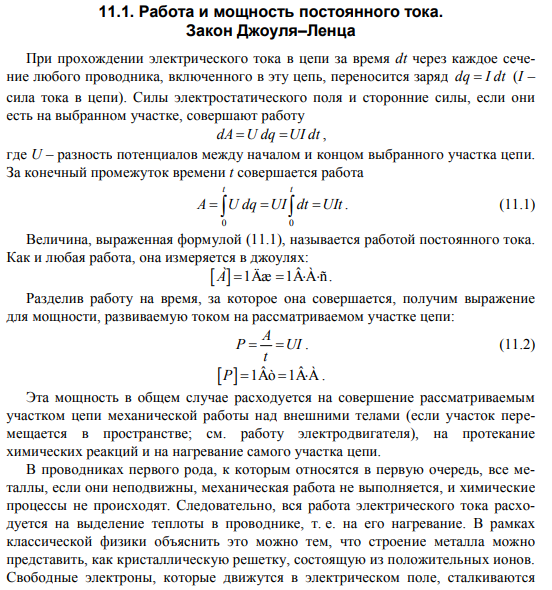
\includegraphics[width=0.5\linewidth]{imgs/q31i2.png}
\end{figure}

\begin{figure}[h]
    \centering
    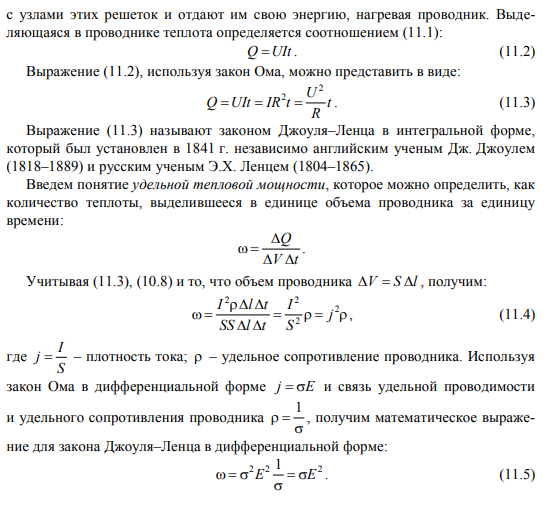
\includegraphics[width=0.5\linewidth]{imgs/q31i3.png}
\end{figure}



